\section{The Lamp of Trismegistus}

According to \textbf{Eliphas Levi} in \emph{Transcendental Magic} the initiate possesses

\begin{itemize}
\item the lamp of Hermes Trismegistus, or reason illuminated by science. 
\item the mantle of Apollonius, of full and complete self-possession, which isolates the sage from blind tendencies 
\item the staff of the patriarchs, which is the help of the secret and everlasting forces of Nature 
\end{itemize}
The lamp of Trismegistus:

\begin{itemize}
\item enlightens present, past, and future 
\item lays bare the conscience of men 
\item manifests the inmost recesses of the female heart 
\end{itemize}
For commentary, please visit Meditations on the Tarot\footnote{\url{https://www.meditationsonthetarot.com/lamp-of-trismegistus}}.

\paragraph{Comment}
The Hermit has given up personal opinions and goals. And he speaks the truth, when necessary, and charitably if possible. But sometimes the objectivity and plain-spokenness is interpreted as rudeness by others. In his role as prophet, he may announce blessings and woes, but the woes are warnings and should be interpreted as kindness, not as rudeness.

\begin{wrapfigure}{rt}{.3\textwidth}
 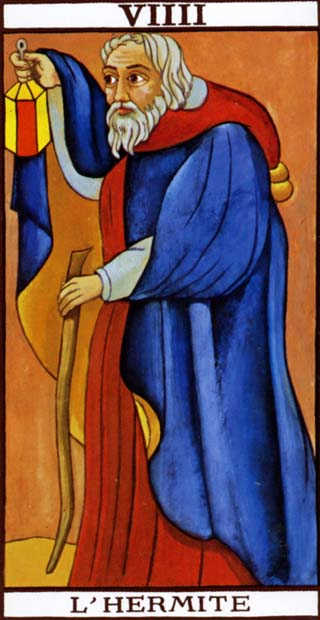
\includegraphics[scale=2.5]{a20100911TheLampofTrismegistus-img001.jpg} 
 \caption{The Hermit} 
\end{wrapfigure}

The Hermit is not really a misanthrope. He loves humanity, but objectively and intellectually, not sentimentally. But humanity prefers sentiment, or the illusion of love, to real love. The lamp with three flames that brings wisdom also casts shadows. So ``the consciences of men are laid bare" and the faults, foibles, pretenses, and illusions of humanity are exposed. So that objective knowledge is not the result of hatred but rather of wisdom (another word for prudence). On the contrary, the mass of men, whom \textbf{Louis Claude de St Martin} called ``men of the torrent", refuse to understand, accept, and integrate their shadows … they are the real haters.

In \emph{La Vita Nuova}, \textbf{Dante} describes his first glimpse, at nine years of age, of his beloved Beatrice, also nine years old. Nine days later at nine o'clock, she greets him on the street. \textbf{Josephin Paladin} in his essay on Dante relates that number to the Hermit, showing again that Dante was an initiate.



\flrightit{Posted on 2010-09-11 by Cologero }
